\section{3. Логістична регресія}

\markright{Частина 3}

Перейдемо до задачі бінарної класифікації. Визначимо цільову змінну:

\[Y_i=\begin{cases}1, & \text{якщо } \mathrm{SalePrice}>130000\\0, & \text{в іншому випадку.}\end{cases}\]


\pythoncode{logit-data}

\Needspace{56pt}
\begingroup\fontsize{7.5}{9.5}\selectfont\setlength{\tabcolsep}{2.5mm}\renewcommand{\arraystretch}{1.12}\par\noindent\begin{tabular}{|lll|}
\hline
Клас & Навчальна & Валідаційна \\
\hline
0 & 627 & 148 \\
1 & 1717 & 438 \\
\hline
\end{tabular}
\par\endgroup


\Needspace{74.39999999999999pt}

\resulttext{p3-c3-out1.txt}

\Needspace{147pt}
\begingroup\fontsize{7.5}{9.5}\selectfont\setlength{\tabcolsep}{2.5mm}\renewcommand{\arraystretch}{1.12}\par\noindent\begin{tabular}{|ll|}
\hline
 & Заповнено медіаною у навчальній частині \\
\hline
Lot\allowbreak{}Frontage & 393 \\
Mas\allowbreak{}Vnr\allowbreak{}Area & 19 \\
Bsmt\allowbreak{}Fin\allowbreak{}SF1 & 1 \\
Bsmt\allowbreak{}Fin\allowbreak{}SF2 & 1 \\
Bsmt\allowbreak{}Unf\allowbreak{}SF & 1 \\
Bsmt\allowbreak{}Full\allowbreak{}Bath & 1 \\
Bsmt\allowbreak{}Half\allowbreak{}Bath & 1 \\
Garage\allowbreak{}Cars & 1 \\
Garage\allowbreak{}Area & 1 \\
\hline
\end{tabular}
\par\endgroup


\Needspace{235pt}

\subsection{3.а Відбір за AIC}

\begin{taskstatement}Оцініть логістичну регресію, використовуючи покроковий зворотний відбір
(Backward Selection) за інформаційним критерієм AIC. Для реалізації
цього алгоритму та зручного розрахунку AIC використовуйте модуль
statsmodels.formula.api.logit або sm.Logit. Щоб прискорити обчислення,
почніть покроковий відбір лише з числових ознак (features). Надалі
аналізуйте виключно фінальну підібрану модель.
\end{taskstatement}

\pythoncode{p3-c6}

\Needspace{147pt}
\begingroup\fontsize{7.5}{9.5}\selectfont\setlength{\tabcolsep}{2.5mm}\renewcommand{\arraystretch}{1.12}\par\noindent\begin{tabular}{|llll|}
\hline
Крок & Вилучено & Ознак & AIC \\
\hline
0 & Початкова модель & 32 & 975.48311 \\
1 & Misc\allowbreak{}Val & 31 & 973.60217 \\
2 & Open\allowbreak{}Porch\allowbreak{}SF & 30 & 971.72607 \\
3 & Tot\allowbreak{}Rms\allowbreak{}Abv\allowbreak{}Grd & 29 & 969.91267 \\
4 & Bedroom\allowbreak{}Abv\allowbreak{}Gr & 28 & 968.06524 \\
5 & Mo\allowbreak{}Sold & 27 & 966.41001 \\
6 & Mas\allowbreak{}Vnr\allowbreak{}Area & 26 & 964.86476 \\
7 & 3Ssn\allowbreak{}Porch & 25 & 963.71709 \\
8 & Low\allowbreak{}Qual\allowbreak{}Fin\allowbreak{}SF & 24 & 963.12802 \\
\hline
\end{tabular}
\par\endgroup


\resulttext{p3-c6-out1.txt}

\Needspace{95pt}
\begingroup\fontsize{7.5}{9.5}\selectfont\setlength{\tabcolsep}{2.5mm}\renewcommand{\arraystretch}{1.12}\par\noindent\begin{tabular}{|ll|}
\hline
 & Значення \\
\hline
Частка |y-p| < 0.0001 & 0.19837884 \\
Максимальний модуль градієнта & 5.3290705e-14 \\
Найменше власне значення інформаційної матриці & 8.7662306 \\
Максимальна різниця коефіцієнтів Newton і BFGS & 1.2407918e-07 \\
Різниця log-likelihood Newton і BFGS & 5.0590643e-12 \\
\hline
\end{tabular}
\par\endgroup


\begingroup\fontsize{7.5}{9.5}\selectfont\setlength{\tabcolsep}{2.5mm}\renewcommand{\arraystretch}{1.12}
\begin{longtable}{|llll|}
\hline
 & Коефіцієнт у початкових одиницях & Стандартна похибка & p-значення \\
\hline
\endfirsthead
\hline
 & Коефіцієнт у початкових одиницях & Стандартна похибка & p-значення \\
\hline
\endhead
\hline\endfoot
Lot\allowbreak{}Frontage & 0.020470732 & 0.0066260011 & 0.002005241 \\
Lot\allowbreak{}Area & 7.9491266e-05 & 3.2299513e-05 & 0.013852448 \\
Overall\allowbreak{}Qual & 0.81739431 & 0.12537262 & 7.0438966e-11 \\
Overall\allowbreak{}Cond & 0.74800588 & 0.098873607 & 3.8704935e-14 \\
Year\allowbreak{}Built & 0.04919673 & 0.0055143401 & 4.5960498e-19 \\
Year\allowbreak{}Remod\allowbreak{}Add & 0.017700964 & 0.0049495669 & 0.00034853813 \\
Bsmt\allowbreak{}Fin\allowbreak{}SF1 & 0.002641284 & 0.0004767892 & 3.0293639e-08 \\
Bsmt\allowbreak{}Fin\allowbreak{}SF2 & 0.0023383025 & 0.00065487033 & 0.00035611781 \\
Bsmt\allowbreak{}Unf\allowbreak{}SF & 0.0019714091 & 0.00039104058 & 4.6203265e-07 \\
1st\allowbreak{}Flr\allowbreak{}SF & 0.004114672 & 0.00058539937 & 2.0827438e-12 \\
2nd\allowbreak{}Flr\allowbreak{}SF & 0.0042424299 & 0.00051338588 & 1.4131057e-16 \\
Bsmt\allowbreak{}Full\allowbreak{}Bath & 0.89737154 & 0.22490109 & 6.6053266e-05 \\
Bsmt\allowbreak{}Half\allowbreak{}Bath & 0.5101582 & 0.33907794 & 0.13244096 \\
Full\allowbreak{}Bath & 0.6857339 & 0.26809045 & 0.010532292 \\
Half\allowbreak{}Bath & 0.47773137 & 0.23618601 & 0.043104991 \\
Kitchen\allowbreak{}Abv\allowbreak{}Gr & -2.3075442 & 0.41753967 & 3.2663239e-08 \\
Fireplaces & 0.61245528 & 0.1663517 & 0.00023169371 \\
Garage\allowbreak{}Cars & 0.43007773 & 0.2677032 & 0.10815381 \\
Garage\allowbreak{}Area & 0.0014827435 & 0.00096385208 & 0.12396265 \\
Wood\allowbreak{}Deck\allowbreak{}SF & 0.0021723264 & 0.00083278367 & 0.009093675 \\
Enclosed\allowbreak{}Porch & 0.0025260833 & 0.0013616231 & 0.063567669 \\
Screen\allowbreak{}Porch & 0.0085011718 & 0.0023399359 & 0.0002800593 \\
Pool\allowbreak{}Area & -0.005498648 & 0.0024770838 & 0.026431873 \\
Yr\allowbreak{}Sold & -0.10616134 & 0.06450283 & 0.09979671 \\
\end{longtable}
\endgroup


\Needspace{19.2pt}

\resulttext{p3-c6-out4.txt}

\answerheading
Для логістичної регресії оцінюємо коефіцієнти методом максимальної
правдоподібності через \texttt{sm.Logit}. Критерій \(AIC=-2\ell+2k\)
поєднує відповідність даним і штраф за складність. Тут \(\ell\) є
логарифмом правдоподібності оціненої моделі, а \(k\) кількістю
параметрів разом із вільним членом.

Починаємо з усіх підготовлених числових ознак. На кожному кроці по черзі
вилучаємо по одній ознаці й повторно оцінюємо модель. Приймаємо
вилучення з найменшим AIC, якщо він нижчий за поточний. Коли жодне таке
вилучення не знижує AIC, зупиняємося. Вільний член зберігаємо на всіх
кроках.

\texttt{summary()} показує коефіцієнти стандартизованих ознак. Для
подальшої інтерпретації повертаємо їх у початкові одиниці за формулами
\(b_j=\widehat\beta_j/s_j\) та
\(b_0=\widehat\beta_0-\sum_j b_j\bar x_j\). Тут \(\widehat\beta_j\) і
\(\widehat\beta_0\) є коефіцієнтом ознаки \(j\) та вільним членом після
стандартизації, \(s_j\) і \(\bar x_j\) її навчальним масштабом і
середнім, а \(b_j\) і \(b_0\) відповідними коефіцієнтами в початкових
одиницях.

Відбір залишив 24 із 32 ознак. AIC зменшився з 975.48311 до 963.12802.
Найкраще наступне вилучення дало б AIC 963.44427, тому відбір зупинився.
Оптимізація досягла збіжності в усіх 253 оцінюваннях, включно з
початковою моделлю.

\texttt{summary()} попереджає про можливе квазірозділення через велику
частку прогнозів, близьких до фактичних 0 або 1. Newton і BFGS дали
практично однакові оцінки: найбільша абсолютна різниця коефіцієнтів
становила близько \(1.24\cdot10^{-7}\).


\Needspace{275pt}

\subsection{3.б Відношення шансів}

\begin{taskstatement}Розгляньте коефіцієнт біля змінної LotArea. Його не можна інтерпретувати
лінійно. Наведіть правильну економічну інтерпретацію через відношення
шансів (Odds Ratio), експоненціювавши коефіцієнт:
\(\exp(\beta_{\mathrm{LotArea}})\).
\end{taskstatement}

\pythoncode{p3-c9}

\Needspace{56pt}
\begingroup\fontsize{7.5}{9.5}\selectfont\setlength{\tabcolsep}{1.5mm}\renewcommand{\arraystretch}{1.12}\par\noindent\begin{tabular}{|>{\raggedright\arraybackslash}p{28.49mm}>{\raggedright\arraybackslash}p{23.57mm}>{\raggedright\arraybackslash}p{23.57mm}>{\raggedright\arraybackslash}p{22.00mm}>{\raggedright\arraybackslash}p{24.32mm}>{\raggedright\arraybackslash}p{25.05mm}|}
\hline
Приріст площі, кв. футів & beta на 1 кв. фут & Відношення шансів & Зміна шансів, \% & Нижня межа OR, 95\% & Верхня межа OR, 95\% \\
\hline
1 & 7.9491266e-05 & 1.0000795 & 0.0079494425 & 1.0000162 & 1.0001428 \\
1000 & 7.9491266e-05 & 1.0827361 & 8.2736103 & 1.0163171 & 1.1534958 \\
\hline
\end{tabular}
\par\endgroup


\answerheading
Шанси ціни понад 130000 доларів дорівнюють \(p/(1-p)\), де \(p\) є
ймовірністю перевищення цього порогу. За незмінних інших ознак приріст
площі ділянки множить шанси на \(OR=e^{db}\), де \(OR\) є відношенням
шансів, \(d\) приростом площі у квадратних футах, а \(b\) коефіцієнтом
\texttt{LotArea} на один квадратний фут. Тут \(e\) є основою
натурального логарифма.

Додатковий квадратний фут множить шанси на 1.0000795. Додаткові 1000
квадратних футів множать їх на 1.0827361, тобто збільшують шанси
приблизно на 8.27\% за незмінних інших ознак.


\Needspace{220pt}

\subsection{3.в Значущість і знаки}

\begin{taskstatement}Сформуйте списки змінних, які статистично значуще збільшують ймовірність
події \(Y = 1\) (додатній коефіцієнт), та тих, що її зменшують
(від'ємний коефіцієнт). Чи узгоджуються ці знаки з базовою економічною
логікою ринку нерухомості?
\end{taskstatement}

\pythoncode{p3-c12}

\Needspace{19.2pt}

\resulttext{p3-c12-out0.txt}

\Needspace{251pt}
\begingroup\fontsize{7.5}{9.5}\selectfont\setlength{\tabcolsep}{2.5mm}\renewcommand{\arraystretch}{1.12}\par\noindent\begin{tabular}{|llll|}
\hline
 & Коефіцієнт у початкових одиницях & Стандартна похибка & p-значення \\
\hline
Lot\allowbreak{}Frontage & 0.020470732 & 0.0066260011 & 0.002005241 \\
Lot\allowbreak{}Area & 7.9491266e-05 & 3.2299513e-05 & 0.013852448 \\
Overall\allowbreak{}Qual & 0.81739431 & 0.12537262 & 7.0438966e-11 \\
Overall\allowbreak{}Cond & 0.74800588 & 0.098873607 & 3.8704935e-14 \\
Year\allowbreak{}Built & 0.04919673 & 0.0055143401 & 4.5960498e-19 \\
Year\allowbreak{}Remod\allowbreak{}Add & 0.017700964 & 0.0049495669 & 0.00034853813 \\
Bsmt\allowbreak{}Fin\allowbreak{}SF1 & 0.002641284 & 0.0004767892 & 3.0293639e-08 \\
Bsmt\allowbreak{}Fin\allowbreak{}SF2 & 0.0023383025 & 0.00065487033 & 0.00035611781 \\
Bsmt\allowbreak{}Unf\allowbreak{}SF & 0.0019714091 & 0.00039104058 & 4.6203265e-07 \\
1st\allowbreak{}Flr\allowbreak{}SF & 0.004114672 & 0.00058539937 & 2.0827438e-12 \\
2nd\allowbreak{}Flr\allowbreak{}SF & 0.0042424299 & 0.00051338588 & 1.4131057e-16 \\
Bsmt\allowbreak{}Full\allowbreak{}Bath & 0.89737154 & 0.22490109 & 6.6053266e-05 \\
Full\allowbreak{}Bath & 0.6857339 & 0.26809045 & 0.010532292 \\
Half\allowbreak{}Bath & 0.47773137 & 0.23618601 & 0.043104991 \\
Fireplaces & 0.61245528 & 0.1663517 & 0.00023169371 \\
Wood\allowbreak{}Deck\allowbreak{}SF & 0.0021723264 & 0.00083278367 & 0.009093675 \\
Screen\allowbreak{}Porch & 0.0085011718 & 0.0023399359 & 0.0002800593 \\
\hline
\end{tabular}
\par\endgroup


\Needspace{19.2pt}

\resulttext{p3-c12-out2.txt}

\Needspace{56pt}
\begingroup\fontsize{7.5}{9.5}\selectfont\setlength{\tabcolsep}{2.5mm}\renewcommand{\arraystretch}{1.12}\par\noindent\begin{tabular}{|llll|}
\hline
 & Коефіцієнт у початкових одиницях & Стандартна похибка & p-значення \\
\hline
Kitchen\allowbreak{}Abv\allowbreak{}Gr & -2.3075442 & 0.41753967 & 3.2663239e-08 \\
Pool\allowbreak{}Area & -0.005498648 & 0.0024770838 & 0.026431873 \\
\hline
\end{tabular}
\par\endgroup


\Needspace{28.4pt}

\resulttext{p3-c12-out4.txt}

\Needspace{56pt}
\begingroup\fontsize{7.5}{9.5}\selectfont\setlength{\tabcolsep}{2.5mm}\renewcommand{\arraystretch}{1.12}\par\noindent\begin{tabular}{|lll|}
\hline
Above130000 & 0 & 1 \\
\hline
False & 626 & 1706 \\
True & 1 & 11 \\
\hline
\end{tabular}
\par\endgroup


\answerheading
Логістична функція зростає, тому за незмінних інших ознак знак
коефіцієнта визначає напрям зміни прогнозованої ймовірності класу 1. У
таблицях наведено ознаки з додатними й від'ємними коефіцієнтами та
\(p\)-значеннями меншими за 0.05. Ці \(p\)-значення умовні для
відібраної моделі й не враховують відбір за AIC.

Додатні коефіцієнти узгоджуються з ринковою логікою: за інших рівних
умов якісніші, краще збережені, більші або новіші будинки частіше
перевищують ціновий поріг. Значущі від'ємні коефіцієнти мають
\texttt{KitchenAbvGr} і \texttt{PoolArea}. Це умовні зв'язки в моделі.
Результат для \texttt{PoolArea} варто тлумачити обережно, бо лише 12
навчальних будинків мають додатну площу басейну.


\Needspace{356pt}

\subsection{3.г П’ять прогнозів}

\begin{taskstatement}Візьміть випадкові 5 будинків із вибірки та розрахуйте для них
ймовірність належати до класу 1 за допомогою методу .predict(). Запишіть
повну математичну формулу логістичної функції \(p=\frac{1}{1+e^{-z}}\)
для першого будинку, підставивши туди реальні значення його ознак та
оцінені моделлю коефіцієнти. Який найпростіший спосіб перейти від
ймовірностей до безпосереднього прогнозу класу (класичний поріг cutoff)?
\end{taskstatement}

\pythoncode{p3-c15}

\Needspace{95pt}
\begingroup\fontsize{7.5}{9.5}\selectfont\setlength{\tabcolsep}{2.5mm}\renewcommand{\arraystretch}{1.12}\par\noindent\begin{tabular}{|lllll|}
\hline
Order & Sale\allowbreak{}Price & Фактичний клас & P(Y=1) & Клас за порогом 0.5 \\
\hline
2925 & 131000 & 1 & 0.9995753 & 1 \\
2360 & 138800 & 1 & 0.69015745 & 1 \\
433 & 610000 & 1 & 1 & 1 \\
1717 & 204000 & 1 & 0.995987 & 1 \\
765 & 159900 & 1 & 0.52943987 & 1 \\
\hline
\end{tabular}
\par\endgroup


\begingroup\fontsize{7.5}{9.5}\selectfont\setlength{\tabcolsep}{2.5mm}\renewcommand{\arraystretch}{1.12}
\begin{longtable}{|llll|}
\hline
 & Значення ознаки & Коефіцієнт & Добуток \\
\hline
\endfirsthead
\hline
 & Значення ознаки & Коефіцієнт & Добуток \\
\hline
\endhead
\hline\endfoot
Lot\allowbreak{}Frontage & 160 & 0.020470732 & 3.2753171 \\
Lot\allowbreak{}Area & 20000 & 7.9491266e-05 & 1.5898253 \\
Overall\allowbreak{}Qual & 5 & 0.81739431 & 4.0869716 \\
Overall\allowbreak{}Cond & 7 & 0.74800588 & 5.2360412 \\
Year\allowbreak{}Built & 1960 & 0.04919673 & 96.42559 \\
Year\allowbreak{}Remod\allowbreak{}Add & 1996 & 0.017700964 & 35.331123 \\
Bsmt\allowbreak{}Fin\allowbreak{}SF1 & 1224 & 0.002641284 & 3.2329316 \\
Bsmt\allowbreak{}Fin\allowbreak{}SF2 & 0 & 0.0023383025 & 0 \\
Bsmt\allowbreak{}Unf\allowbreak{}SF & 0 & 0.0019714091 & 0 \\
1st\allowbreak{}Flr\allowbreak{}SF & 1224 & 0.004114672 & 5.0363585 \\
2nd\allowbreak{}Flr\allowbreak{}SF & 0 & 0.0042424299 & 0 \\
Bsmt\allowbreak{}Full\allowbreak{}Bath & 1 & 0.89737154 & 0.89737154 \\
Bsmt\allowbreak{}Half\allowbreak{}Bath & 0 & 0.5101582 & 0 \\
Full\allowbreak{}Bath & 1 & 0.6857339 & 0.6857339 \\
Half\allowbreak{}Bath & 0 & 0.47773137 & 0 \\
Kitchen\allowbreak{}Abv\allowbreak{}Gr & 1 & -2.3075442 & -2.3075442 \\
Fireplaces & 1 & 0.61245528 & 0.61245528 \\
Garage\allowbreak{}Cars & 2 & 0.43007773 & 0.86015545 \\
Garage\allowbreak{}Area & 576 & 0.0014827435 & 0.85406024 \\
Wood\allowbreak{}Deck\allowbreak{}SF & 474 & 0.0021723264 & 1.0296827 \\
Enclosed\allowbreak{}Porch & 0 & 0.0025260833 & 0 \\
Screen\allowbreak{}Porch & 0 & 0.0085011718 & 0 \\
Pool\allowbreak{}Area & 0 & -0.005498648 & -0 \\
Yr\allowbreak{}Sold & 2006 & -0.10616134 & -212.95964 \\
\end{longtable}
\endgroup


\Needspace{37.599999999999994pt}

\resulttext{p3-c15-out2.txt}

\Needspace{530pt}

Повна підстановка для першого будинку (порядок ознак як у таблиці;
показані числа округлено):

\[\begin{aligned}z &\approx 63.8772652416\\& +0.020470732147\cdot 160\\& +0.000079491266\cdot 20000\\& +0.817394310330\cdot 5\\& +0.748005880712\cdot 7\\& +0.049196729518\cdot 1960\\& +0.017700963663\cdot 1996\\& +0.002641283975\cdot 1224\\& +0.002338302470\cdot 0\\& +0.001971409081\cdot 0\\& +0.004114671961\cdot 1224\\& +0.004242429923\cdot 0\\& +0.897371535405\cdot 1\\& +0.510158195409\cdot 0\\& +0.685733903603\cdot 1\\& +0.477731367771\cdot 0\\& -2.307544158146\cdot 1\\& +0.612455279815\cdot 1\\& +0.430077726125\cdot 2\\& +0.001482743473\cdot 576\\& +0.002172326428\cdot 474\\& +0.002526083256\cdot 0\\& +0.008501171822\cdot 0\\& -0.005498647983\cdot 0\\& -0.106161336239\cdot 2006\\&\approx 7.76369829251\end{aligned}\]

\[p=\frac{1}{1+e^{-(7.76369829251)}}\approx 0.999575298116.\]


\answerheading
За стандартного порогу прогнозуємо клас 1, якщо \(p\ge0.5\), і клас 0
інакше. Тут \(p\) є прогнозованою ймовірністю ціни понад 130000 доларів.

У виводі наведено ймовірності \texttt{.predict()} для п'яти випадково
вибраних будинків і повну числову підстановку для першого. Для будинку
\texttt{Order=2925} показник \(z\), тобто сума вільного члена й добутків
коефіцієнтів на значення ознак, становить приблизно 7.7636983, а
ймовірність 0.9995753, тому прогнозуємо клас 1. Фактична ціна цього
будинку становить 131000 доларів. Усі п'ять випадково вибраних будинків
цього разу належать до класу 1.


\Needspace{299pt}

\subsection{3.д Матриця помилок при 0.5}

\begin{taskstatement}Побудуйте матрицю помилок за допомогою функції confusion\_matrix з
sklearn.metrics для стандартного порогу 0.5. Розрахуйте чутливість
(recall / sensitivity), специфічність та загальну точність (accuracy).
Надайте розгорнуту словесну інтерпретацію кожної клітинки матриці
помилок у контексті вартості та доступності будинків.
\end{taskstatement}

\pythoncode{p3-c18}

\Needspace{56pt}
\begingroup\fontsize{7.5}{9.5}\selectfont\setlength{\tabcolsep}{2.5mm}\renewcommand{\arraystretch}{1.12}\par\noindent\begin{tabular}{|lll|}
\hline
 & Прогноз 0 & Прогноз 1 \\
\hline
Факт 0 & 125 & 23 \\
Факт 1 & 19 & 419 \\
\hline
\end{tabular}
\par\endgroup


\Needspace{147pt}
\begingroup\fontsize{7.5}{9.5}\selectfont\setlength{\tabcolsep}{2.5mm}\renewcommand{\arraystretch}{1.12}\par\noindent\begin{tabular}{|ll|}
\hline
 & Значення \\
\hline
Поріг & 0.5 \\
TN & 125 \\
FP & 23 \\
FN & 19 \\
TP & 419 \\
Чутливість & 0.956621 \\
Специфічність & 0.84459459 \\
Accuracy & 0.92832765 \\
Прогнозів класу 1 & 442 \\
\hline
\end{tabular}
\par\endgroup


\Needspace{19.2pt}

\resulttext{p3-c18-out2.txt}

\begin{figure}[H]\centering
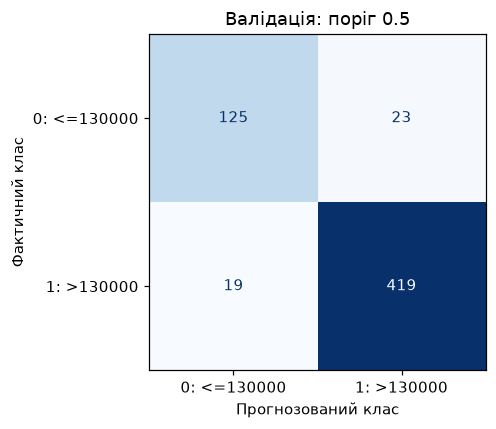
\includegraphics[width=0.52\linewidth,height=0.85\textheight,keepaspectratio]{../../figures/part3_confusion_default.png}
\caption{Матриця помилок при порозі 0.5.}
\end{figure}

\answerheading
У матриці рядки відповідають фактичному класу, а стовпці прогнозованому.
Чутливість дорівнює \(TP/(TP+FN)\), специфічність \(TN/(TN+FP)\), а
загальна точність \((TP+TN)/N\). Тут \(TP\) і \(TN\) є кількостями
правильних прогнозів класів 1 і 0, \(FP\) і \(FN\) кількостями хибних
прогнозів цих класів, а \(N\) кількістю валідаційних будинків.

\begin{itemize}
\item
  TN (125). Фактична ціна вкладається в бюджет 130000 доларів, і модель
  правильно визначила ці будинки як доступні за цим порогом.
\item
  FP (23). Фактична ціна вкладається в бюджет, але модель спрогнозувала
  дорожчу групу. Покупець із таким бюджетом може помилково відкинути ці
  будинки.
\item
  FN (19). Фактична ціна перевищує бюджет, але модель спрогнозувала
  доступну групу. Покупець може помилково очікувати, що ці будинки
  вкладаються в бюджет.
\item
  TP (419). Фактична ціна перевищує бюджет, і модель правильно віднесла
  ці будинки до дорожчої групи.
\end{itemize}

За порогу 0.5 чутливість становить 0.9566, специфічність 0.8446, а
загальна точність 0.9283.


\Needspace{266pt}

\subsection{3.е ROC та поріг Юдена}

\begin{taskstatement}Оскільки поріг 0.5 не завжди є оптимальним, побудуйте ROC-криву за
допомогою roc\_curve та знайдіть площу під нею (roc\_auc\_score).
Визначте оптимальний поріг класифікації, максимізувавши індекс Юдена
(Sensitivity+Specificity−1). Побудуйте графік кривої за допомогою
matplotlib.
\end{taskstatement}

\pythoncode{p3-c21}

\Needspace{95pt}
\begingroup\fontsize{7.5}{9.5}\selectfont\setlength{\tabcolsep}{2.5mm}\renewcommand{\arraystretch}{1.12}\par\noindent\begin{tabular}{|ll|}
\hline
 & Значення \\
\hline
ROC AUC & 0.97280328 \\
Поріг Юдена & 0.67279019 \\
Індекс Юдена & 0.84129335 \\
Чутливість & 0.92237443 \\
Специфічність & 0.91891892 \\
\hline
\end{tabular}
\par\endgroup


\begin{figure}[H]\centering
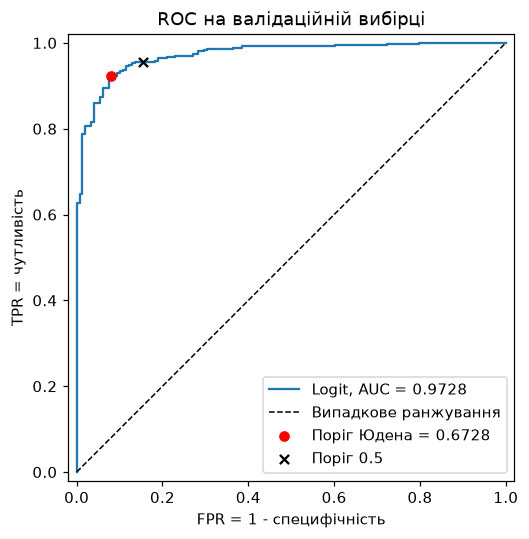
\includegraphics[width=0.6\linewidth,height=0.85\textheight,keepaspectratio]{../../figures/part3_roc.png}
\caption{ROC-крива й обраний поріг Юдена.}
\end{figure}

\answerheading
ROC показує, як чутливість і частка хибнопозитивних прогнозів змінюються
з порогом. AUC є площею під цією кривою та характеризує, наскільки добре
модель ранжує будинки двох класів.

Вибираємо поріг, що максимізує \(J=\mathrm{TPR}-\mathrm{FPR}\). Тут
\(J\) є індексом Юдена, \(\mathrm{TPR}\) чутливістю, а \(\mathrm{FPR}\)
часткою хибнопозитивних прогнозів серед будинків класу 0. Оскільки
\(\mathrm{FPR}\) дорівнює одиниці мінус специфічність, цей критерій дає
однакову вагу чутливості та специфічності.

AUC на валідаційній вибірці становить 0.9728. Найбільший індекс Юдена
0.8413 отримали за порогу 0.6728. Оскільки поріг вибрано на цій самій
вибірці, метрики за ним описують результат на даних, використаних для
вибору порогу.


\Needspace{211pt}

\subsection{3.ж Класифікація з новим порогом}

\begin{taskstatement}Перерахуйте матрицю помилок, чутливість та специфічність для нового
(оптимального за ROC) порогу. Порівняйте ці метрики з отриманими при
порозі 0.5. Дайте відповідь: чи стала ваша модель після зміни порогу
більш «консервативною» щодо прогнозування дорогих будинків (клас 1)?
\end{taskstatement}

\pythoncode{p3-c24}

\Needspace{147pt}
\begingroup\fontsize{7.5}{9.5}\selectfont\setlength{\tabcolsep}{2.5mm}\renewcommand{\arraystretch}{1.12}\par\noindent\begin{tabular}{|lll|}
\hline
 & Стандартний & За Юденом \\
\hline
Поріг & 0.5 & 0.67279019 \\
TN & 125 & 136 \\
FP & 23 & 12 \\
FN & 19 & 34 \\
TP & 419 & 404 \\
Чутливість & 0.956621 & 0.92237443 \\
Специфічність & 0.84459459 & 0.91891892 \\
Accuracy & 0.92832765 & 0.92150171 \\
Прогнозів класу 1 & 442 & 416 \\
\hline
\end{tabular}
\par\endgroup


\Needspace{56pt}
\begingroup\fontsize{7.5}{9.5}\selectfont\setlength{\tabcolsep}{2.5mm}\renewcommand{\arraystretch}{1.12}\par\noindent\begin{tabular}{|lll|}
\hline
 & Прогноз 0 & Прогноз 1 \\
\hline
Факт 0 & 136 & 12 \\
Факт 1 & 34 & 404 \\
\hline
\end{tabular}
\par\endgroup


\Needspace{28.4pt}

\resulttext{p3-c24-out2.txt}

\begin{figure}[H]\centering
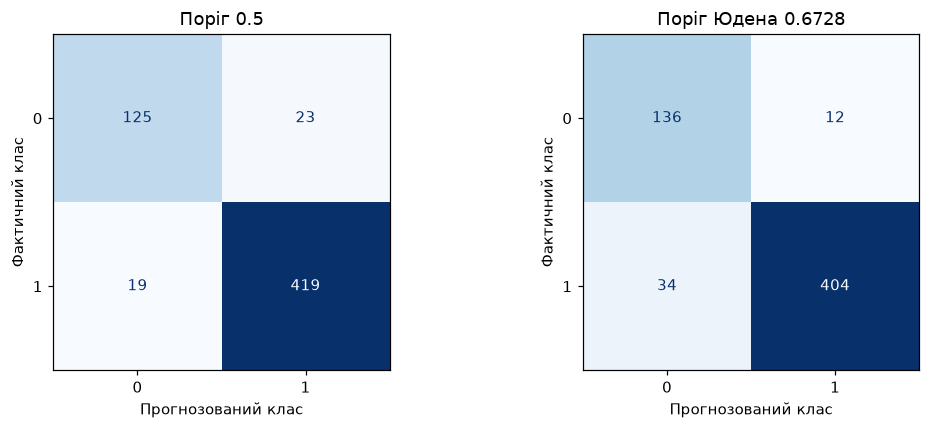
\includegraphics[width=0.85\linewidth,height=0.85\textheight,keepaspectratio]{../../figures/part3_confusion_comparison.png}
\caption{Порівняння матриць помилок для двох порогів.}
\end{figure}

\answerheading
Змінюємо лише поріг перетворення ймовірності на клас. За вищого порогу
моделі потрібна більша прогнозована ймовірність, щоб віднести будинок до
класу 1.

Правило стало більш консервативним щодо дорогих будинків. Поріг зріс із
0.5 до 0.6728, і кількість прогнозів класу 1 зменшилася з 442 до 416.
Хибнопозитивних прогнозів стало 12 замість 23, а хибнонегативних 34
замість 19. Специфічність зросла з 0.8446 до 0.9189, а чутливість
зменшилася з 0.9566 до 0.9224. Модель рідше помилково називає доступний
будинок дорогим, але частіше пропускає справді дорогі будинки.

